\subsection{Tracing and profiling}

\begin{frame}[fragile]{strace}
  \begin{columns}
  \column{0.75\textwidth}
  \small
  System call tracer - \url{https://strace.io}
  \begin{itemize}
  \item Available on all GNU/Linux systems\\
        Can be built by your cross-compiling toolchain generator or by your build system.
  \item Allows to see what any of your processes is doing: accessing files, allocating memory...
        Often sufficient to find simple bugs.
  \item Usage:\\
    \code{strace <command>} (starting a new process)\\
    \code{strace -f <command>} ({\bf f}ollow child processes too)\\
    \code{strace -p <pid>} (tracing an existing process)\\
    \code{strace -c <command>} (time statistics per system call)
    \code{strace -e <expr> <command>} (use {\bf e}xpression for advanced filtering)
  \end{itemize}
  See \href{https://man7.org/linux/man-pages/man1/strace.1.html}{the strace manual} for details.
  \column{0.25\textwidth}
  
\includegraphics[height=0.7\textheight]{slides/linux-app-tracing/strace-mascot.png}\\
  \tiny Image credits: \url{https://strace.io/}
  \end{columns}
\end{frame}

\begin{frame}[fragile]{strace example output}
  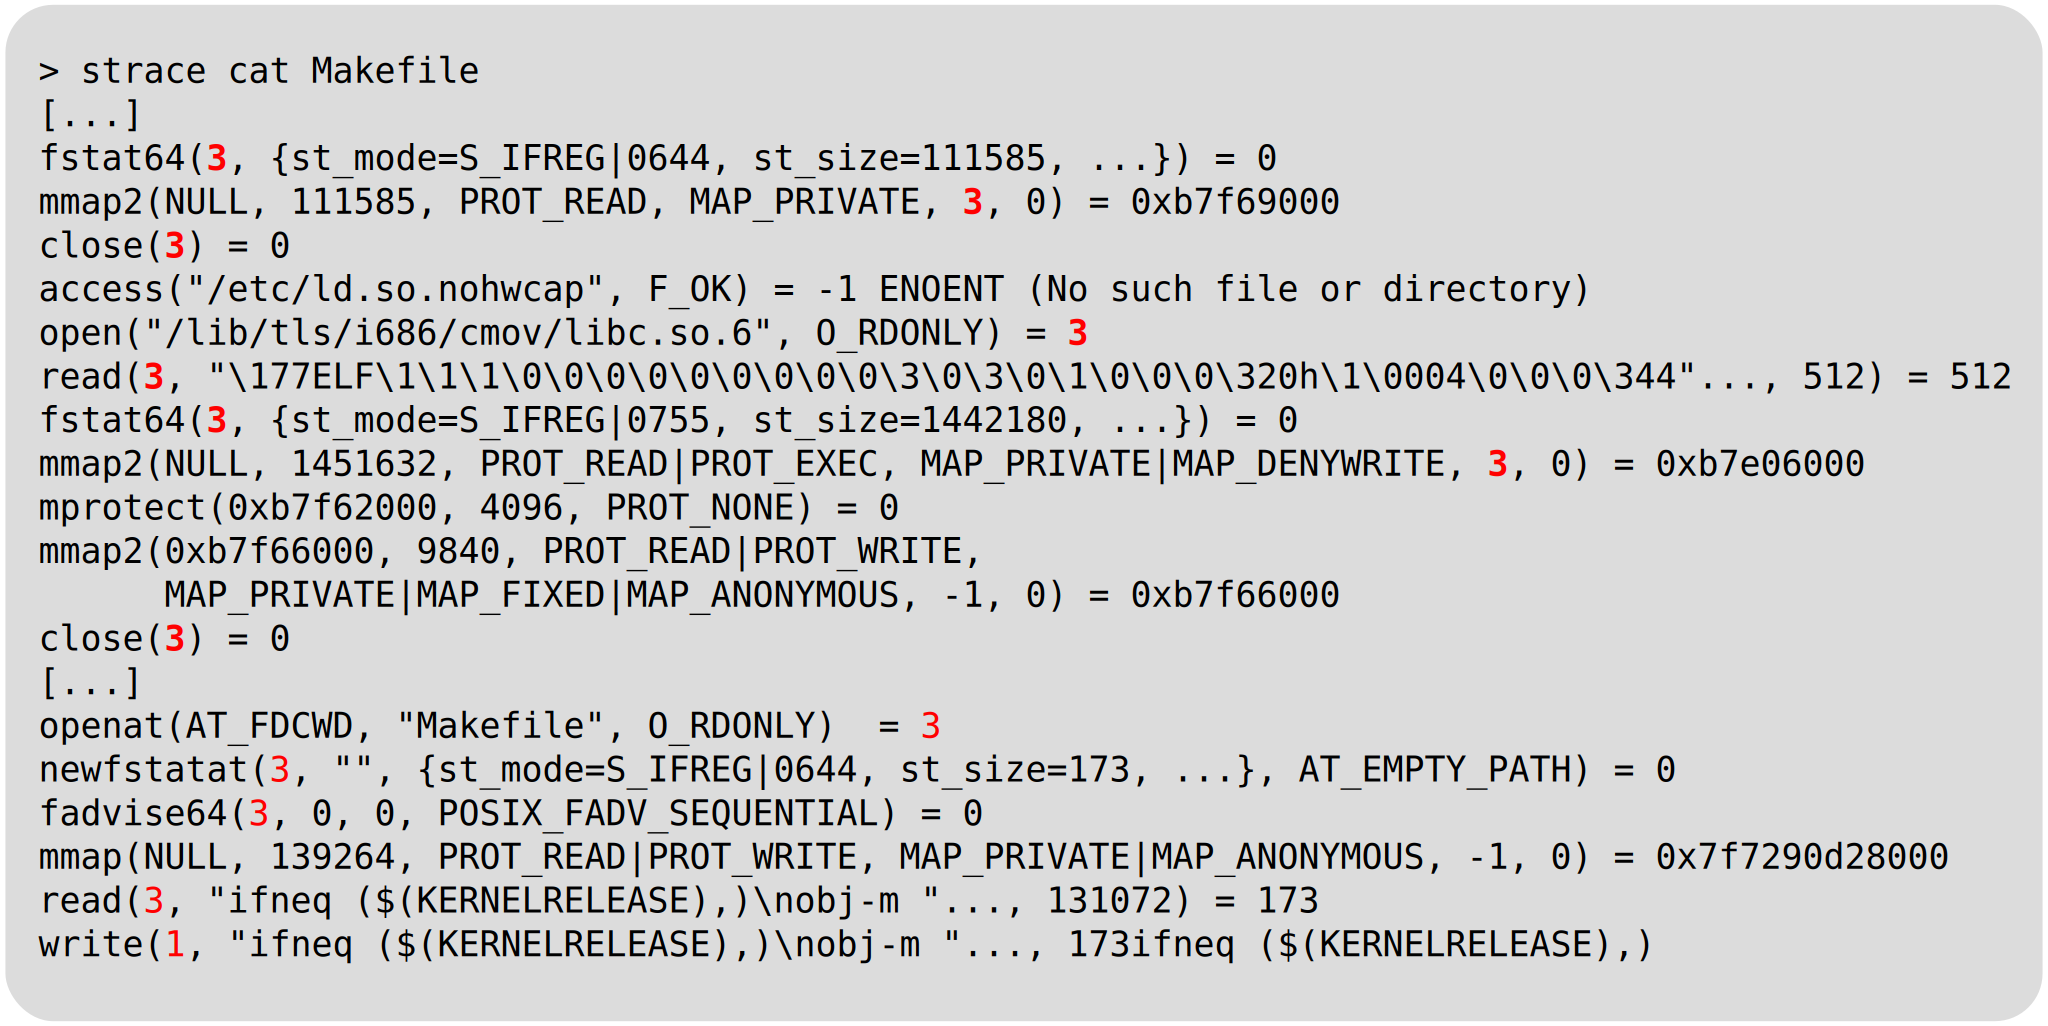
\includegraphics[height=0.75\textheight]{slides/linux-app-tracing/strace-output.pdf}\\
  Hint: follow the open file descriptors returned by \code{open()}.
  This tells you what files are handled by further system calls.
\end{frame}

\begin{frame}[fragile]
  \frametitle{strace -c example output}
  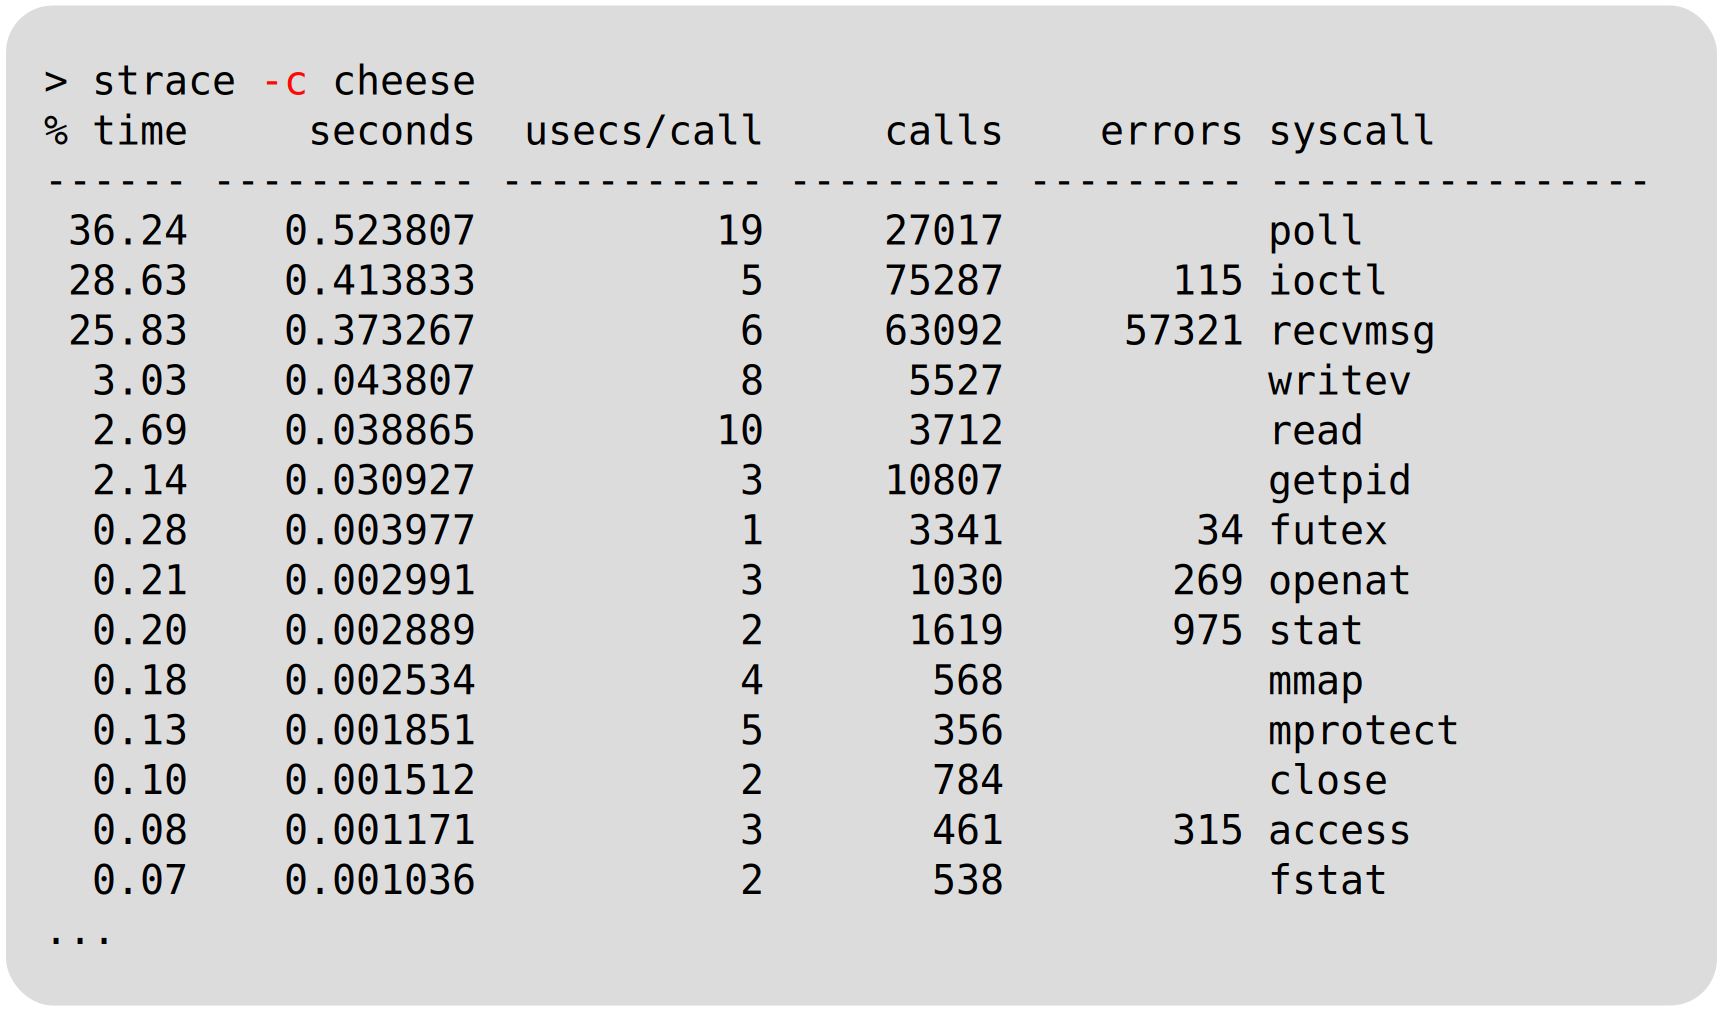
\includegraphics[height=0.8\textheight]{slides/linux-app-tracing/strace-c-output.pdf}
\end{frame}

\begin{frame}{ltrace}
  A tool to trace {\bf shared} library calls used by a program and all the signals
  it receives
  \begin{itemize}
  \item Very useful complement to \code{strace}, which shows only system
    calls.
  \item Of course, works even if you don't have the sources
  \item Allows to filter library calls with regular expressions, or
    just by a list of function names.
  \item With the \code{-S} option it shows system calls too!
  \item Also offers a summary with its \code{-c} option.
  \item Manual page: \url{https://linux.die.net/man/1/ltrace}
  \item Works better with {\em glibc}. \code{ltrace} used to be broken
        with {\em uClibc} (now fixed), and is not supported
        with {\em Musl} (Buildroot 2022.11 status).
  \end{itemize}
  See \url{https://en.wikipedia.org/wiki/Ltrace} for details
\end{frame}

\begin{frame}[fragile]{ltrace example output}
  \scriptsize
  \begin{block}{}
\begin{verbatim}
# ltrace  ffmpeg -f video4linux2 -video_size 544x288 -input_format mjpeg -i /dev
/video0 -pix_fmt rgb565le -f fbdev /dev/fb0
__libc_start_main([ "ffmpeg", "-f", "video4linux2", "-video_size"... ] <unfinished ...>
setvbuf(0xb6a0ec80, nil, 2, 0)                   = 0
av_log_set_flags(1, 0, 1, 0)                     = 1
strchr("f", ':')                                 = nil
strlen("f")                                      = 1
strncmp("f", "L", 1)                             = 26
strncmp("f", "h", 1)                             = -2
strncmp("f", "?", 1)                             = 39
strncmp("f", "help", 1)                          = -2
strncmp("f", "-help", 1)                         = 57
strncmp("f", "version", 1)                       = -16
strncmp("f", "buildconf", 1)                     = 4
strncmp("f", "formats", 1)                       = 0
strlen("formats")                                = 7
strncmp("f", "muxers", 1)                        = -7
strncmp("f", "demuxers", 1)                      = 2
strncmp("f", "devices", 1)                       = 2
strncmp("f", "codecs", 1)                        = 3
...
\end{verbatim}
\end{block}
\end{frame}

\begin{frame}[fragile]{ltrace summary}
  Example summary at the end of the ltrace output (\code{-c} option)
  \scriptsize
  \begin{block}{}
\begin{verbatim}

% time     seconds  usecs/call     calls      function
------ ----------- ----------- --------- --------------------
 52.64    5.958660     5958660         1 __libc_start_main
 20.64    2.336331     2336331         1 avformat_find_stream_info
 14.87    1.682895         421      3995 strncmp
  7.17    0.811210      811210         1 avformat_open_input
  0.75    0.085290         584       146 av_freep
  0.49    0.055150         434       127 strlen
  0.29    0.033008         660        50 av_log
  0.22    0.025090         464        54 strcmp
  0.20    0.022836       22836         1 avformat_close_input
  0.16    0.017788         635        28 av_dict_free
  0.15    0.016819         646        26 av_dict_get
  0.15    0.016753         440        38 strchr
  0.13    0.014536         581        25 memset
...
------ ----------- ----------- --------- --------------------
100.00   11.318773                  4762 total
\end{verbatim}
  \end{block}
\end{frame}

\begin{frame}{ftrace}
  \begin{itemize}
  \item In-kernel {\em tracing} functionality
  \item Can trace
    \begin{itemize}
    \item Well-defined trace locations in the kernel, called {\em
        tracepoints}, identifying important events in the kernel:
      scheduling, interrupts, etc.
    \item Arbitrary functions in the kernel
    \item Arbitrary functions in user-space applications
    \end{itemize}
  \item Low-overhead and optimized tracing
  \item Accessible using the dedicated {\em tracefs} filesystem
  \item \code{trace-cmd} is a higher-level CLI tool to use {\em
      ftrace}
  \item Can be used to understand overall system activity (what is my
    system doing?) as well as narrow down specific performance
    issues
  \item \url{https://www.kernel.org/doc/Documentation/trace/ftrace.txt}
  \item \url{https://www.trace-cmd.org/}
  \end{itemize}
\end{frame}

\begin{frame}{kernelshark}
  \begin{itemize}
  \item Visualization tool for {\em ftrace} traces
  \item \url{https://kernelshark.org/}
  \end{itemize}
  \begin{center}
    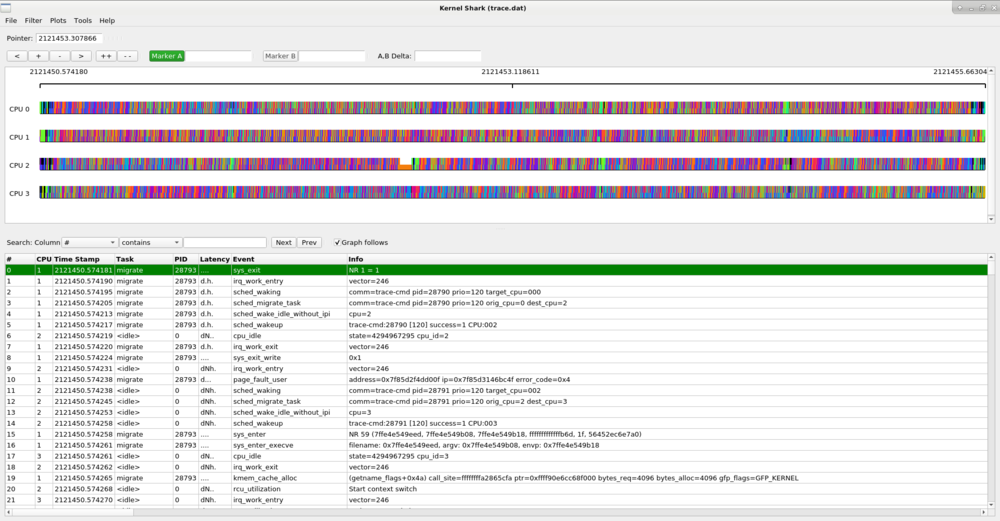
\includegraphics[height=0.6\textheight]{slides/linux-app-tracing/kernelshark.png}
  \end{center}
\end{frame}

\begin{frame}{perf}
  \begin{itemize}
  \item {\em instrument CPU performance counters, tracepoints, kprobes, and uprobes}
  \item Directly included in the Linux kernel source code: \kfile{tools/perf}
  \item Began as a tool for using the performance counters in Linux,
    and has had various enhancements to add tracing capabilities
  \item Supports a list of measurable events: hardware events (cycle
    count, L1 cache hits/miss, page faults), software events
    (tracepoints)
  \item \url{https://perf.wiki.kernel.org}
  \end{itemize}
\end{frame}

\begin{frame}{perf examples}
  \begin{itemize}
  \item List all currently known events\\
    \code{perf list}
  \item List scheduler tracepoints\\
    \code{perf list 'sched:*'}
  \item CPU counter statistics for the specified command\\
    \code{perf stat <command>}
  \item CPU counter statistics for the entire system, for 5 seconds\\
    \code{perf stat -a sleep 5}
  \item Profiling: sample on-CPU functions for the specified command, at 99 Hertz\\
    \code{perf record -F 99 <command>}
  \item Tracing: trace all context-switches via sched tracepoint, until Ctrl-C\\
    \code{perf record -e sched:sched_switch -a}
  \item Many more at \url{https://www.brendangregg.com/perf.html}
  \end{itemize}
\end{frame}

\begin{frame}{perf GUI: hotspot}
  \begin{columns}
    \column{0.4\textwidth}
    \begin{itemize}
    \item Hotspot - the Linux perf GUI for performance analysis
    \item The main feature of hotspot is visualizing a \code{perf.data} file graphically
    \item \href{https://github.com/KDAB/hotspot}{github.com/KDAB/hotspot}
    \end{itemize}
    \column{0.6\textwidth}
    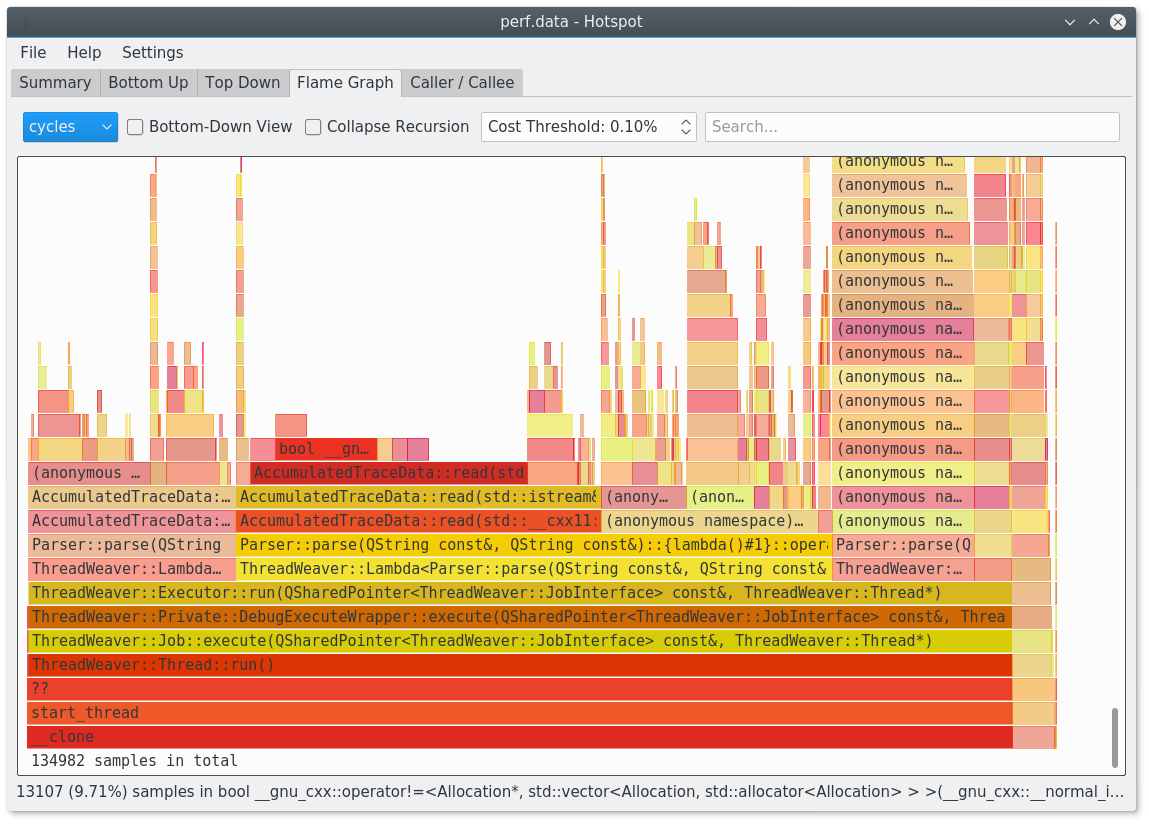
\includegraphics[width=\textwidth]{slides/linux-app-tracing/hotspot.png}
  \end{columns}
\end{frame}

\begin{frame}{gprof}
  \begin{itemize}
  \item Application-level profiler
  \item Part of {\em binutils}
  \item Requires passing gcc \code{-pg} option at build/link time
  \item Run your program normally, it automatically generates a
    \code{gmon.out} file when exiting
  \item Use the \code{gprof} tool on \code{gmon.out} to extract
    profiling data
  \item \url{http://sourceware.org/binutils/docs/gprof/}
  \end{itemize}
\end{frame}

\begin{frame}[fragile]{gprof example}
  \begin{columns}
    \column{0.6\textwidth}
    \begin{block}{}
      {\tiny
\begin{verbatim}
$ ./test-gprof
$ gprof test-gprof gmon.out
Flat profile:

Each sample counts as 0.01 seconds.
  %   cumulative   self              self     total
 time   seconds   seconds    calls   s/call   s/call  name
 35.31      7.46     7.46        1     7.46    13.92  func1
 34.03     14.65     7.19        1     7.19     7.19  func2
 30.57     21.11     6.46        1     6.46     6.46  new_func1
  0.09     21.13     0.02                             main
[...]
\end{verbatim}
      }
    \end{block}
    \column{0.4\textwidth}
    \begin{center}
      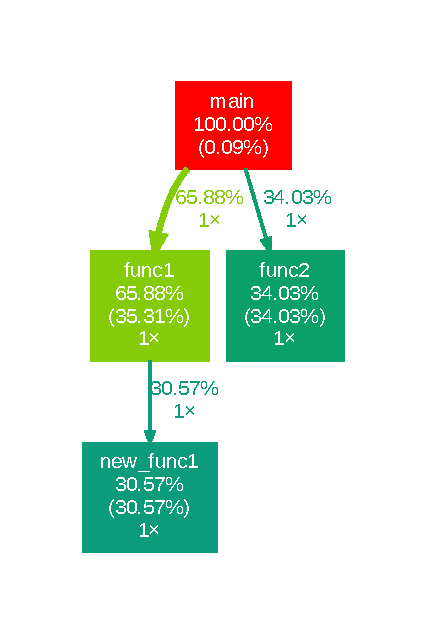
\includegraphics[height=0.6\textheight]{slides/linux-app-tracing/gprof2dot.pdf}\\
      {\small Generated with \href{https://github.com/jrfonseca/gprof2dot}{gprof2dot}}
    \end{center}
  \end{columns}
\end{frame}
